\section{Werkzeuge der Bildverabreitung}
Die folgende Zusammenfassung der Thematik basiert auf dem Buch
"Digitale Bildverarbeitung" von Burger, Burge \citep{BurgeDigitBild}, das als 
Standartliteratur zu empfehlen ist. Eine zusammenfassende Wiedergabe der für 
das Projekt relevanter Themen ist im Folgenden nachzulesen.\\
Ein Bestandteil der Bildverarbeitung ist die Bildanalyse, bei der
sinnvolle Informationen aus Bildern extrahiert werden. Genauer ist der Themenbereich
\textit{Computer Vision} gemeint, bei dem es um das Mechanisieren von
Sehvorgängen des Menschen in der dreidimensionalen Welt geht.\\
Die Steuerung des Wagens soll durch Informationen aus den Kamerabildern
erfolgen: Durch Erkennen der Fahrbahnlinien wird der Lenkungsservo geregelt, der
das Auto innerhalb der Spur zwischen den Fahrpahnlinien hält.\\
Dieser Prozess lässt sich in Einzelschritten beschreiben mit:
\begin{enumerate}
  \item \textit{Digitalisierung} der dreidimensionalen Welt mit Hilfe der Kamera
  \item \textit{Vorverarbeitung} (Bildverbesserung bzw. Anpassung an den Zweck) durch
    Umwandlung in ein binäres Canny-Edges-Bild
  \item \textit{Segmentierung} durch Vorauswahl des Bildauschnittes mit den relevante
    Informationen
  \item \textit{Merkmalsextraktion} zur Linienerkennung durch die Hough-Transformation
  \item \textit{Parametrisierung} als mathematische  Beschreibung der Fahrbahnlinien zur
    weiteren Informationsverarbeitung
\end{enumerate}

\subsection{Digitalisierung}
Der von der Kamera aufgenommen Bilder-Stream liegt in digitaler Form vor. Dabei lassen
sich benötigte Parameter eintellen. Um ein optimales Bild zu
erhalten sind die Beleuchtungsumstände zu beachten, da hierdurch die
Differenzierung von Linien im Bild erheblich beeinflusst wird.\\
Anzumerken ist hier, dass in der Bildverabreitung der Ursprung des
Koordinatensystems bzw. der x- und y-Achse in der linken
oberen Ecke des Bildes definiert ist.

\subsection{Vorverarbeitung - Der Canny-Kantenoperator}
Zur späteren Erkennung der Linien werden die dafür relevanten Informationen aus
dem Bild gefiltert: sogenannte Bildkannten. Bildkanten sind Übergangsstellen, wo
ein hoher Grauwertsprung von einem Pixel zum Nachbarpixel vorliegt, wie z. B. bei 
einem weißen Farbahnstreifen auf dunkler Fahrbahn, hier werden zwei Kannten
analysiert. Kanten werden dem entsprechend an diversen Stellen im Bild
detektiert, deshalb sind die Parameter entsprechend zu wählen.\\
Die Canny-Edges-Funktion ist ein bewährter Algorithmus zur Kantenerkennung, da drei Ziel
gleichzeitig erreicht werden drei Ziele: ein zuverlässiges Detektieren
vorhandener Kanten, die Position der Kante präzise zu bestimmen, und Farbsprünge, 
die nicht als Kante interoretiert werden sollen, auszulassen. Diese Funktion
ist in der OpenCV-Library enthalten. \\

\subsection{Segmentierung}
[BILD Kamera mit Fahrbahnlinien]
Der für die Erkennung der Fahrbahnlinien relevante Bereich liegt in einem
unteren Dreieck des Kamerabildes. Dieser Teil wird ausgewählt, bzw. davon ausserhalb
liegende Bereiche werden nicht bei der Erkennenung der Farbahnlinien
berücksichtigt.\\

\subsection{Merkmalsextraktion zur Linienerkennung}
Das Canny-Kantenbild wird mit Hilfe der Hough-Transformation aus der
openCV-Library in den Hough-Raum transformiert, wo dann die Erkennung der Linien
erfolgt.

\begin{minipage}{\columnwidth}
  \makeatletter
  \def\@captype{figure}
  \makeatother
  \centering
  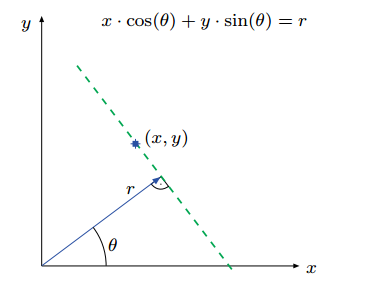
\includegraphics[width=0.8\linewidth]{images/gradeThetaR.png}
  \caption{Beschreibung einer Graden durch Winkel und Abstand vom Ursprung}
  \label{fig:gradeThetaR}
\end{minipage}

Dabei kommt zur Anwendung, dass eine Gerade mathematisch sowohl mit $y
= m \cdot x + b$ als auch mit $r(\theta) = x \cdot cos(\theta) + y \cdot
sin(\theta)$ beschrieben werden kann. Dabei ist in der zweiten Beschreibung 
$\theta$ der  Winkel des Radius $r$ zum Urspung, an dessen Ende senkrecht die
beschriebene Grade verläuft. Zu Bedenken ist, dass wie schon erwähnt der
Koordinatenursprung des Bildes oben links definiert ist.\\
Das rechenaufwendige Verfahren der Hough-Transformation generiert für jeden
Kantenbildpunkt des Canny-Edges-Bildes Bildpunkte im Hough-Raum, dessen Achsen
ein $\theta$ / $r$ - Koordinatensystem bilden. Linien im kartesisches System
sind als Punkthäufungen im Hough-Raum erkennbar. Liegt eine Anzahl von
Punkten oberhalb eines zu definierenden Schwellwertes, wird eine Linie erkannt
und die Houh-Transformationsfunktion gibt ein Wertpaar $\theta$, $r$ zurück.
